\section{ILA-Breaching Effects}\label{sec:ila_effects}

In this section, we present $<>$ effects \todo{add value} identified in the ATMega163 microcontroller that breach ILA and pose a hazard to any masking scheme's security. Analytically, the effects below demonstrate that independent computations \emph{do not} necessairly lead to independent leakages and thus the order-reduction theorem can become applicable.

Every effect (Sections~\ref{overwrite},~\ref{mem_remnant} and~\ref{combined_leakage} $<>$) is described as a standalone, assembly-based scenario that manipulates two 4-bit shares $x_0$, $x_1$ originating from the sensitive, key-dependent, 4-bit value $x$, such that $x=x_0 \oplus x_1$. The shares $x_0$, $x_1$ are always manipulated in a theoretically sound manner, adhering to the masking scheme's requirements, i.e. we never combine the shares directly (e.g. via an exclusive-or instruciton \texttt{eor x0, x1}). 

For all the described scenarios, that should be theoretically sound, we show experimentally that ILA is not fulfilled by employing 1st-order, univariate techniques. Namely, we perform correlation-based analysis~\cite{DBLP:conf/ches/BrierCO04}, computing $\rho$ between the Hamming weight of the sensitive, key-dependent value $x$ and the experimentally acquired traceset. To maintain a wide attack scope, we also use the leakage detection methodology~\cite{tvla,DBLP:conf/ches/SchneiderM15} and compute the 1st-order, random vs. fixed t-test. 
 We conclude every scenario by suggesting possible solutions that enforce ILA and verify all the proposed solutions experimentally, using a large number of traces. Restating Balasch et al.~\cite{DBLP:conf/cardis/BalaschGGRS14}, as we are always limited by the traces at hand, we cannot rule out the existence of 1st-order leakages, yet we establish that their informativeness is limited compared to 2nd-order leakages in the target device. Note that extra care is taken in order to assess all effects independently, i.e. we use the suggested solutions so as to isolate the effect under discussion from the rest.

The effects under discussion can manifest in several data storage units (e.g. registers, SRAM/Flash memory cells, I/O buffers, etc.) and may relate to different instructions of the AVR ISA\footnote{\url{http://www.atmel.com/images/Atmel-0856-AVR-Instruction-Set-Manual.pdf}}, leading to a very large number of potential scenarios. In order to maintain a feasible scope, we limit our discussion to storage instructions and instructions that are often encountered in the context of cryptographic implementation, i.e. logical instructions and SRAM memory accesses.
\begin{subsection}{Overwrite Effect}\label{overwrite}

The overwrite effect is observable when a share gets overwritten by a different share from the same family. For instance, if share $x_0$ in a data storage unit (register, memory cell, etc.) gets overwritten by share $x_1$, then the power consumption correlates with the number of bits switched i.e. $x_0 \oplus x_1$. This effect was observed by Daemen et al.~\cite{noteonsca} and later revisited by Coron et al.~\cite{DBLP:conf/cosade/CoronGPRRV12}.\\
 Below, we address the most common situations in which overwriting arises during a cryptographic implementation. We perform two experiments: a register-based overwrite via the instruction \texttt{mov x0, x1}, and a memory-based overwrite via \texttt{st SRAM\_x0 ,  x1}. 
%Note that overwriting effects can arise due to other instructions and/or storage units. For example, \texttt{ld x0, SRAM\_x1} will cause a similar %effect and it is also subject to the operation remnant effect (see Section \ref{remnant_section}). Overwriting the I/O buffers or partial overwriting via %the \texttt{bld, bst} instructions can produce the same effect (see Appendix A).
\begin{figure}[H]
    \centering
\begin{subfigure}[b]{0.4\textwidth}
      \texttt{;share x0 in r17 \\
;share x1 in r23 \\
\textbf{mov r17,r23}\\
			}

        \caption{\scriptsize{Register overwrite experiment.}}

    \end{subfigure}
 \begin{subfigure}[b]{0.4\textwidth}
         \texttt{;share x0 in SRAM 0x0080 \\
;share x1 in r17  \\
ldi r27,0x00 \\
ldi r26,0x80 \\
st X,r17\\
}

        \caption{\scriptsize{Memory overwrite experiment.}}

    \end{subfigure}

 \begin{subfigure}[b]{0.47\textwidth}
        %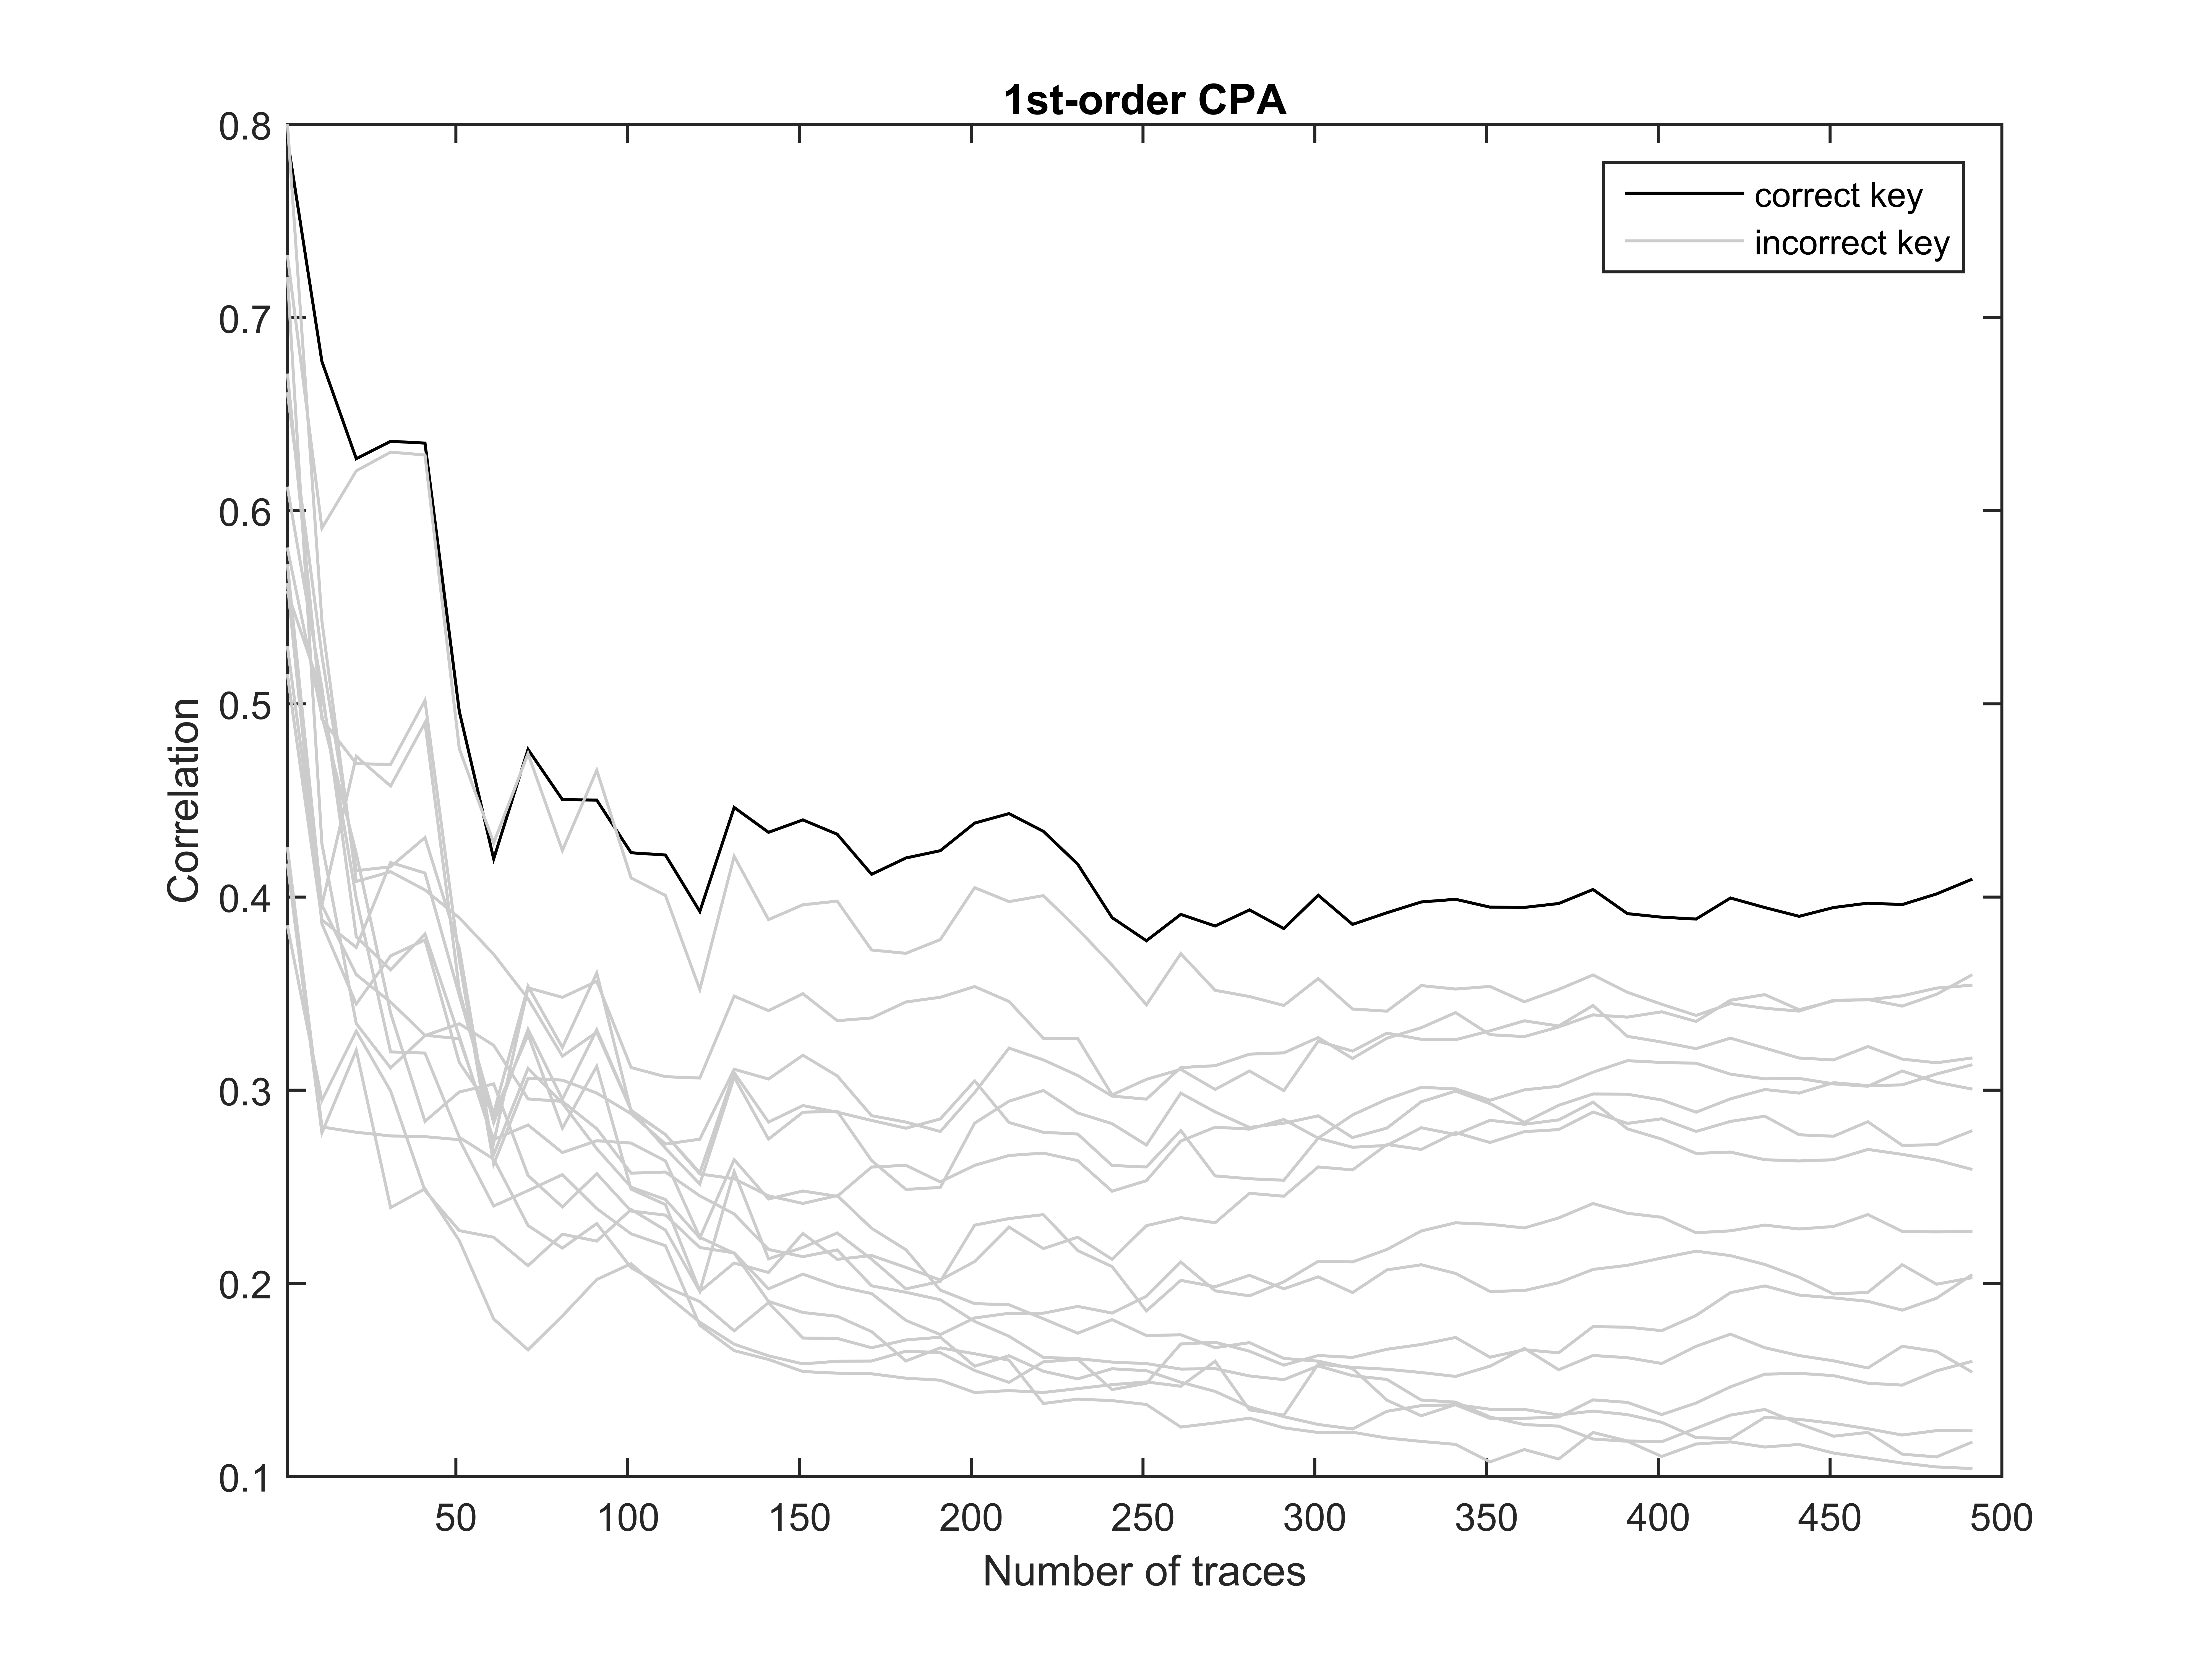
\includegraphics[width=\textwidth]{reg_over_cpa.png}

        \caption{\scriptsize{Register overwrite, 1st-order CPA, HW model, 500 traces.}}

    \end{subfigure}
 \begin{subfigure}[b]{0.47\textwidth}
       %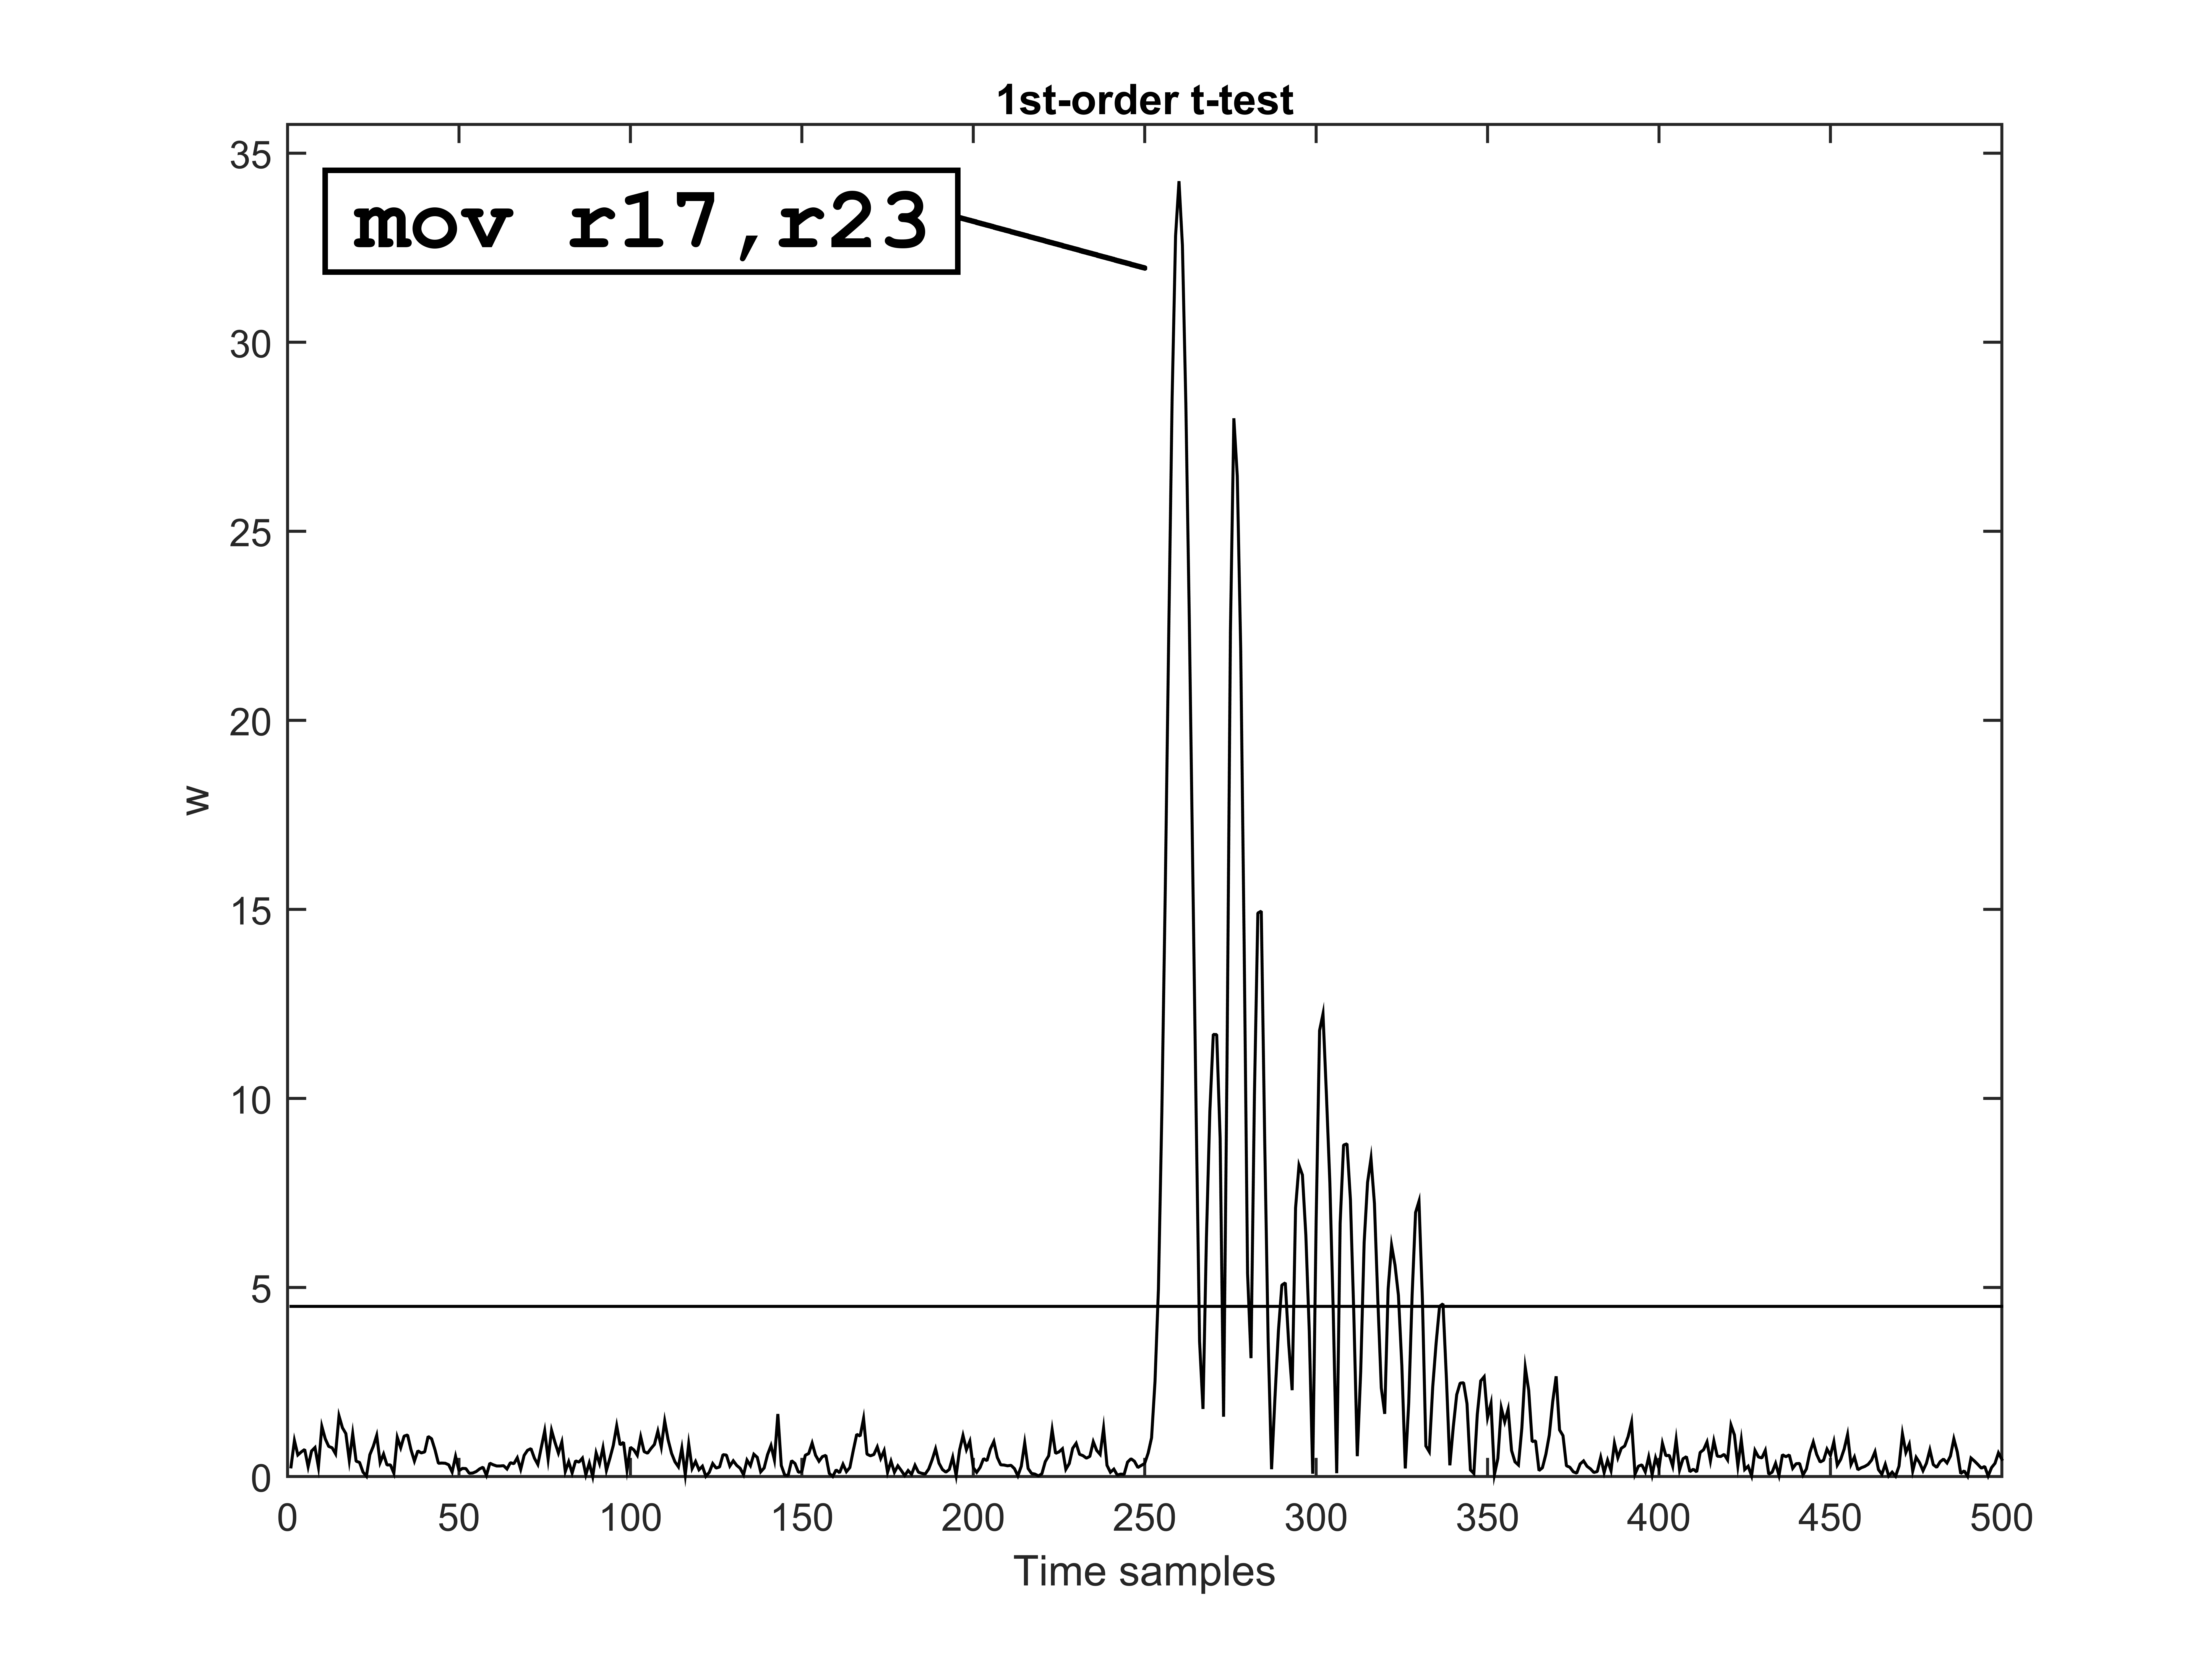
\includegraphics[width=\textwidth]{reg_over_t_an.png}

        \caption{\scriptsize{Register overwrite, 1st-order t-test, 5k random vs. 5k fixed.}}

    \end{subfigure}

     %add desired spacing between images, e. g. ~, \quad, \qquad, \hfill etc. 
      %(or a blank line to force the subfigure onto a new line)
    \begin{subfigure}[b]{0.47\textwidth}
        %\includegraphics[width=\textwidth]{memory_over_cpa.png}
        \caption{\scriptsize{Memory overwrite, 1st-order CPA, HW model, 65k traces.}}
        \label{fig:tiger}
    \end{subfigure}
    %add desired spacing between images, e. g. ~, \quad, \qquad, \hfill etc. 
    %(or a blank line to force the subfigure onto a new line)
    \begin{subfigure}[b]{0.47\textwidth}
        %\includegraphics[width=\textwidth]{memory_over_t_an.png}
        \caption{\scriptsize{Memory overwrite, 1st order t-test, 50k random vs. 50k fixed.}}

    \end{subfigure}
    \caption{Register/memory-based overwrite effects}\label{fig:mem}
\end{figure}
%Causing overwrites is also possible via load/store instructions from/to Flash memory , yet the high computational cost of accessing the Flash memory %makes it less common situation in cryptographic implementations (although it has exhibited potential for AVR and TI-based %microcontrollers~\cite{shuffled, feram}). 
We confirm that overwriting is indeed an ILA-breaching effect, manifesting both in registers and SRAM memory. Note that the exploitability of the effect varies according to the data storage unit: in ATMega163, register-based overwriting can be exploited with roughly 500 traces, while memory-based requires at least 40k traces. Preventing register/memory-based overwrites is straightforward: the corresponding register/cell needs to be cleared in advance. We confirm experimentally that this solution remains secure against a $<>$k \todo{add value} random vs. $<>$k fixed, 1st-order t-test (see Appendix A\todo{add appendix}).
\label{overwrite_section}
\end{subsection}

\begin{subsection}{Memory Remnant Effect} \label{mem_remnant}

The memory remnant effect is a type of leakage originating from consecutive SRAM accesses to different shares of the same family. For instance, assume that shares $x_0$, $x_1$ are stored in SRAM cells and get accessed sequentially. Naturally, the first access leaks share $x_0$ (value-based leakage), yet it also creates a ``remnant" of $x_0$. The second memory access will leak share $x_1$ (value-based leakage) \emph{and} the remnant $x_0$ concurrently, reducing the security order of the scheme.

We address this scenario with the two following experiments. First, we demonstrate how two consecutive SRAM accesses \texttt{ld rA, SRAM\_x0} and \texttt{ld rB, SRAM\_x1} produce the remnant effect. Second, we show how clearing the register and inserting a dummy SRAM access can remove the remnant.    
\begin{figure}[H]
    \centering
\begin{subfigure}[b]{0.4\textwidth}
      \texttt{;share x0 in 0x0080 \\
;share x1 in 0x0090 \\
ldi r27, 0x00\\
ldi r26, 0x80\\
ld r17, X\\
ldi r27, 0x00\\
ldi r26, 0x90\\
ld r20, X
			}

        \caption{\scriptsize{Memory remnant experiment.}}

    \end{subfigure}
\begin{subfigure}[b]{0.4\textwidth}
          \texttt{;share x0 in 0x0080 \\
;share x1 in 0x0090 \\
ldi r27, 0x00\\
ldi r26, 0x80\\
ld r17, X\\
ldi r17, 0x00\\ 
ldi r26, 0x85\\
ld r17, X\\
ldi r26, 0x90\\
ld r20, X
			}
\todo[inline]{should it be r17 in 'ldi r17, 0x00' and in the 2nd 'ld r17, X'?}
        \caption{\scriptsize{Clearing remnant experiment.}}

    \end{subfigure}


 \begin{subfigure}[b]{0.47\textwidth}
        %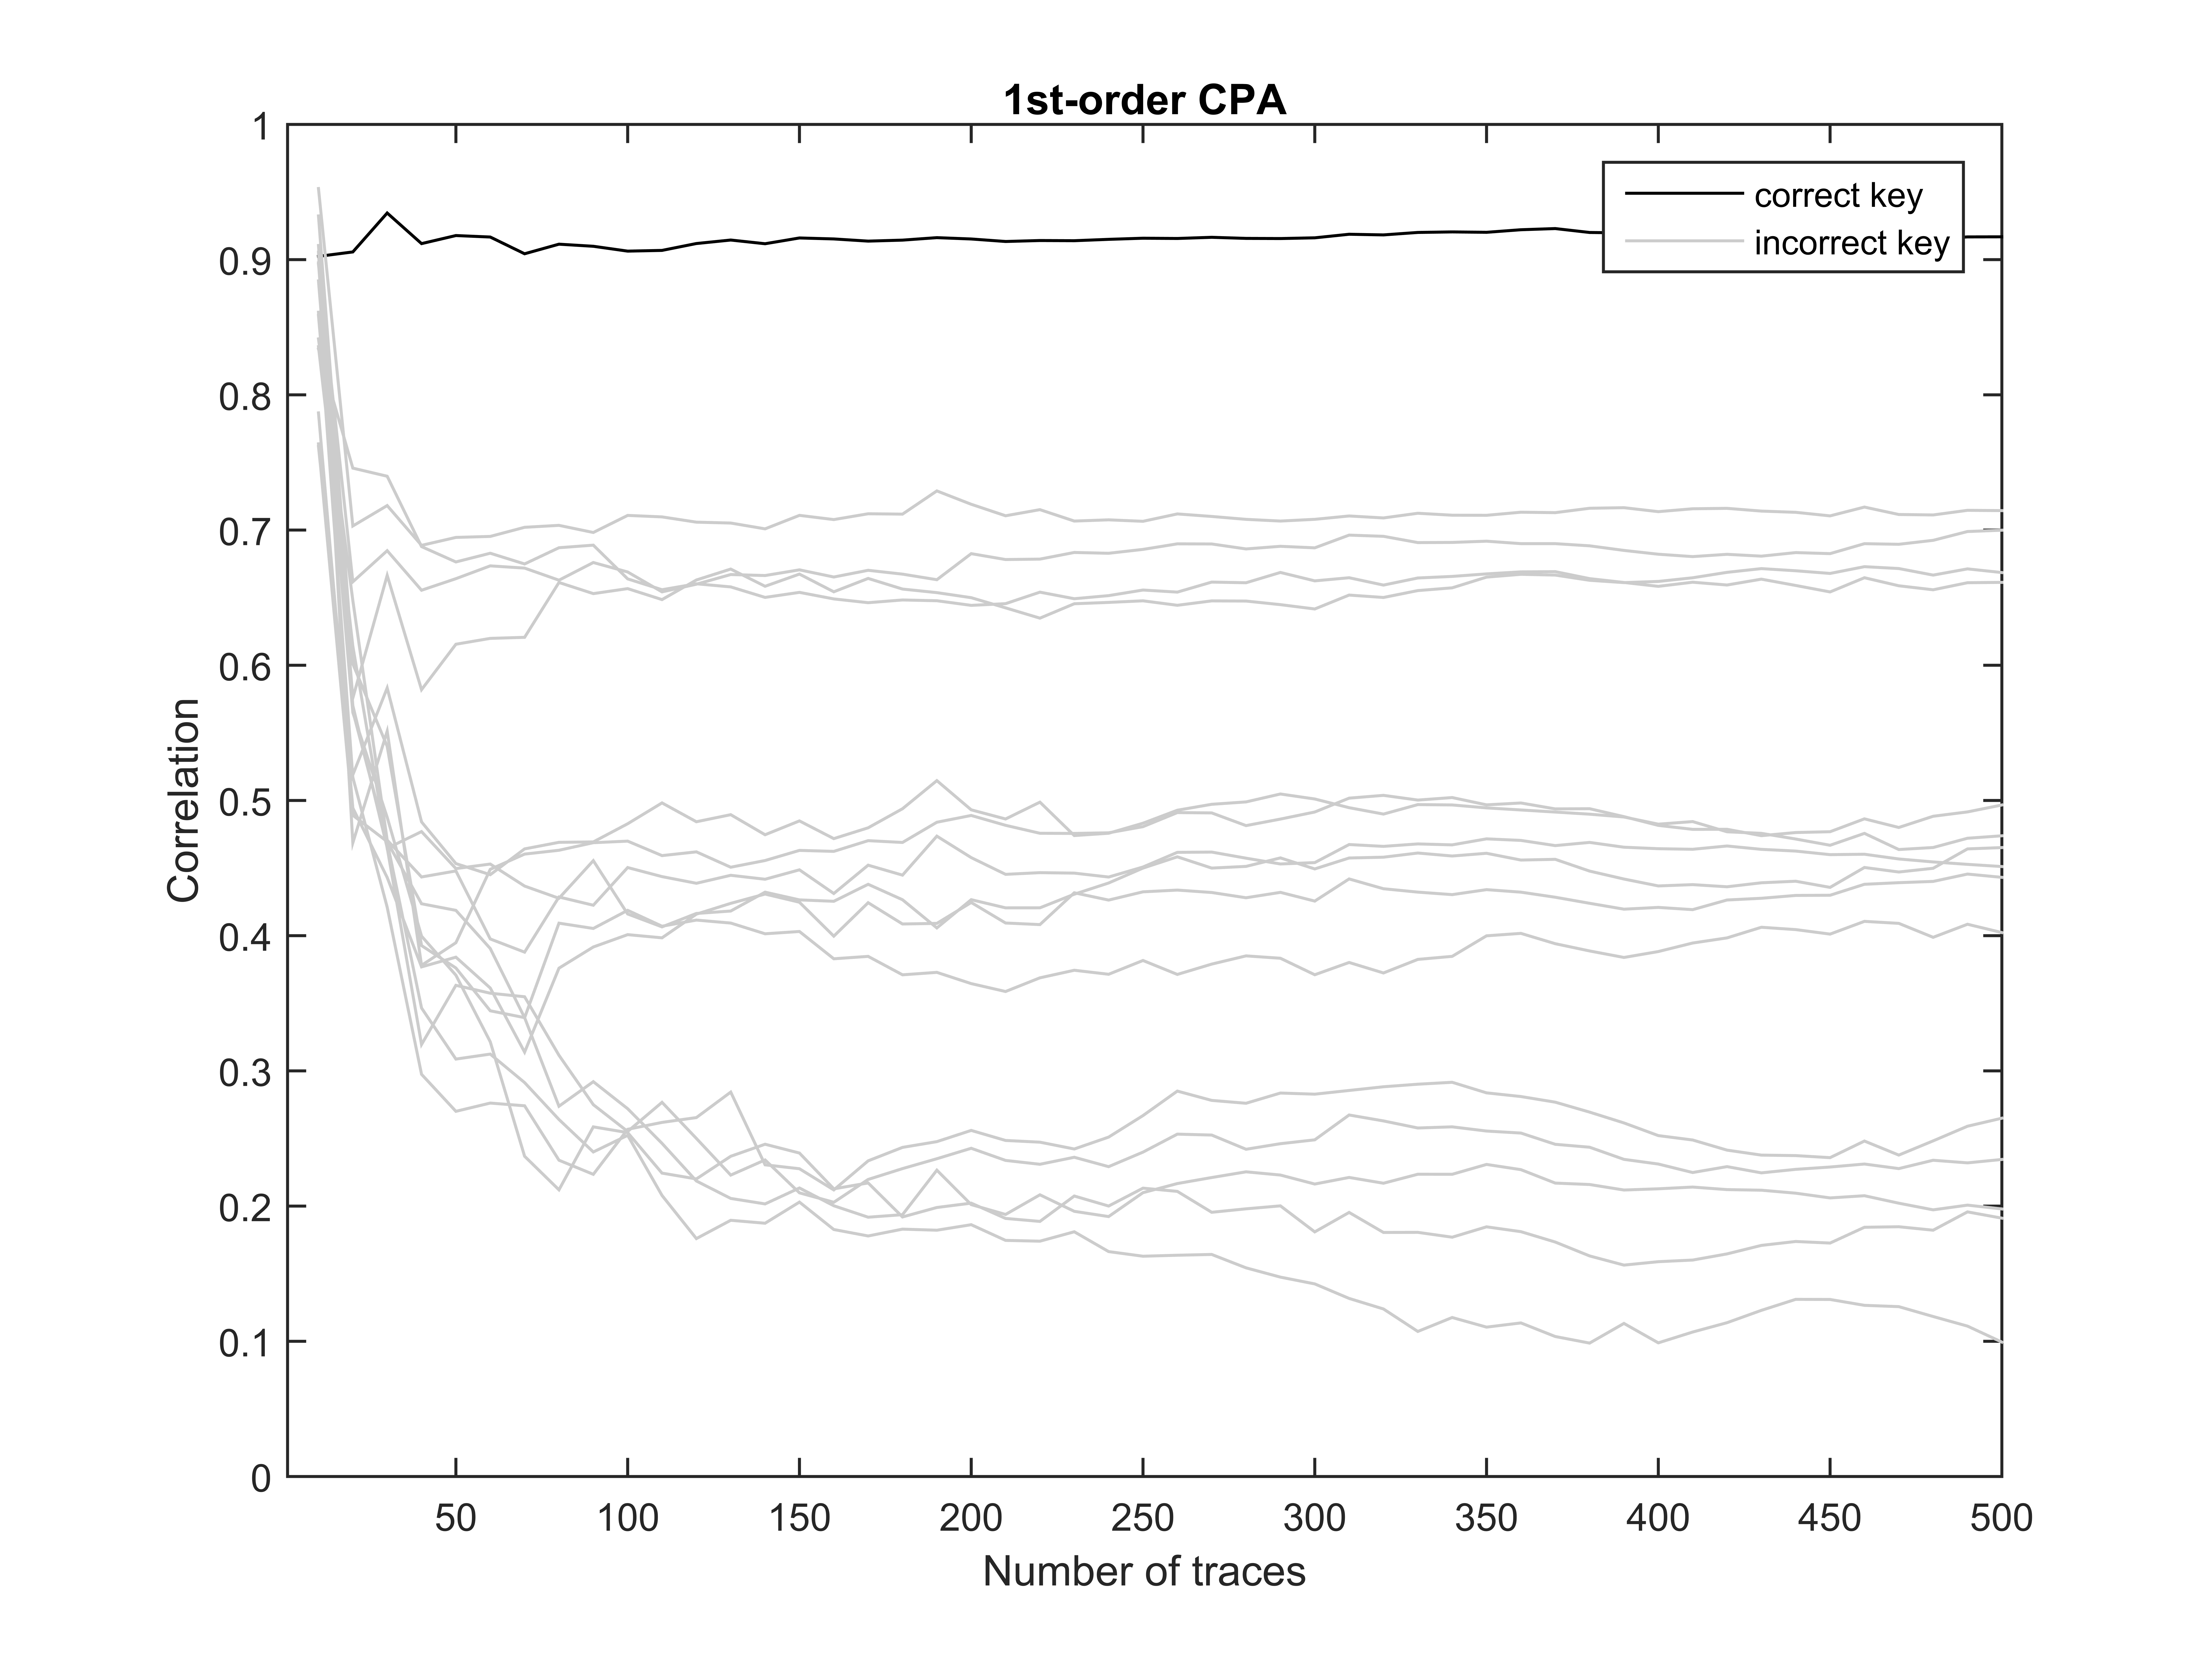
\includegraphics[width=\textwidth]{mem_rem_cpa.png}

        \caption{\scriptsize{Memory remnant effect,1st-order CPA, HW model, 500 traces.}}

    \end{subfigure}
 \begin{subfigure}[b]{0.47\textwidth}
      %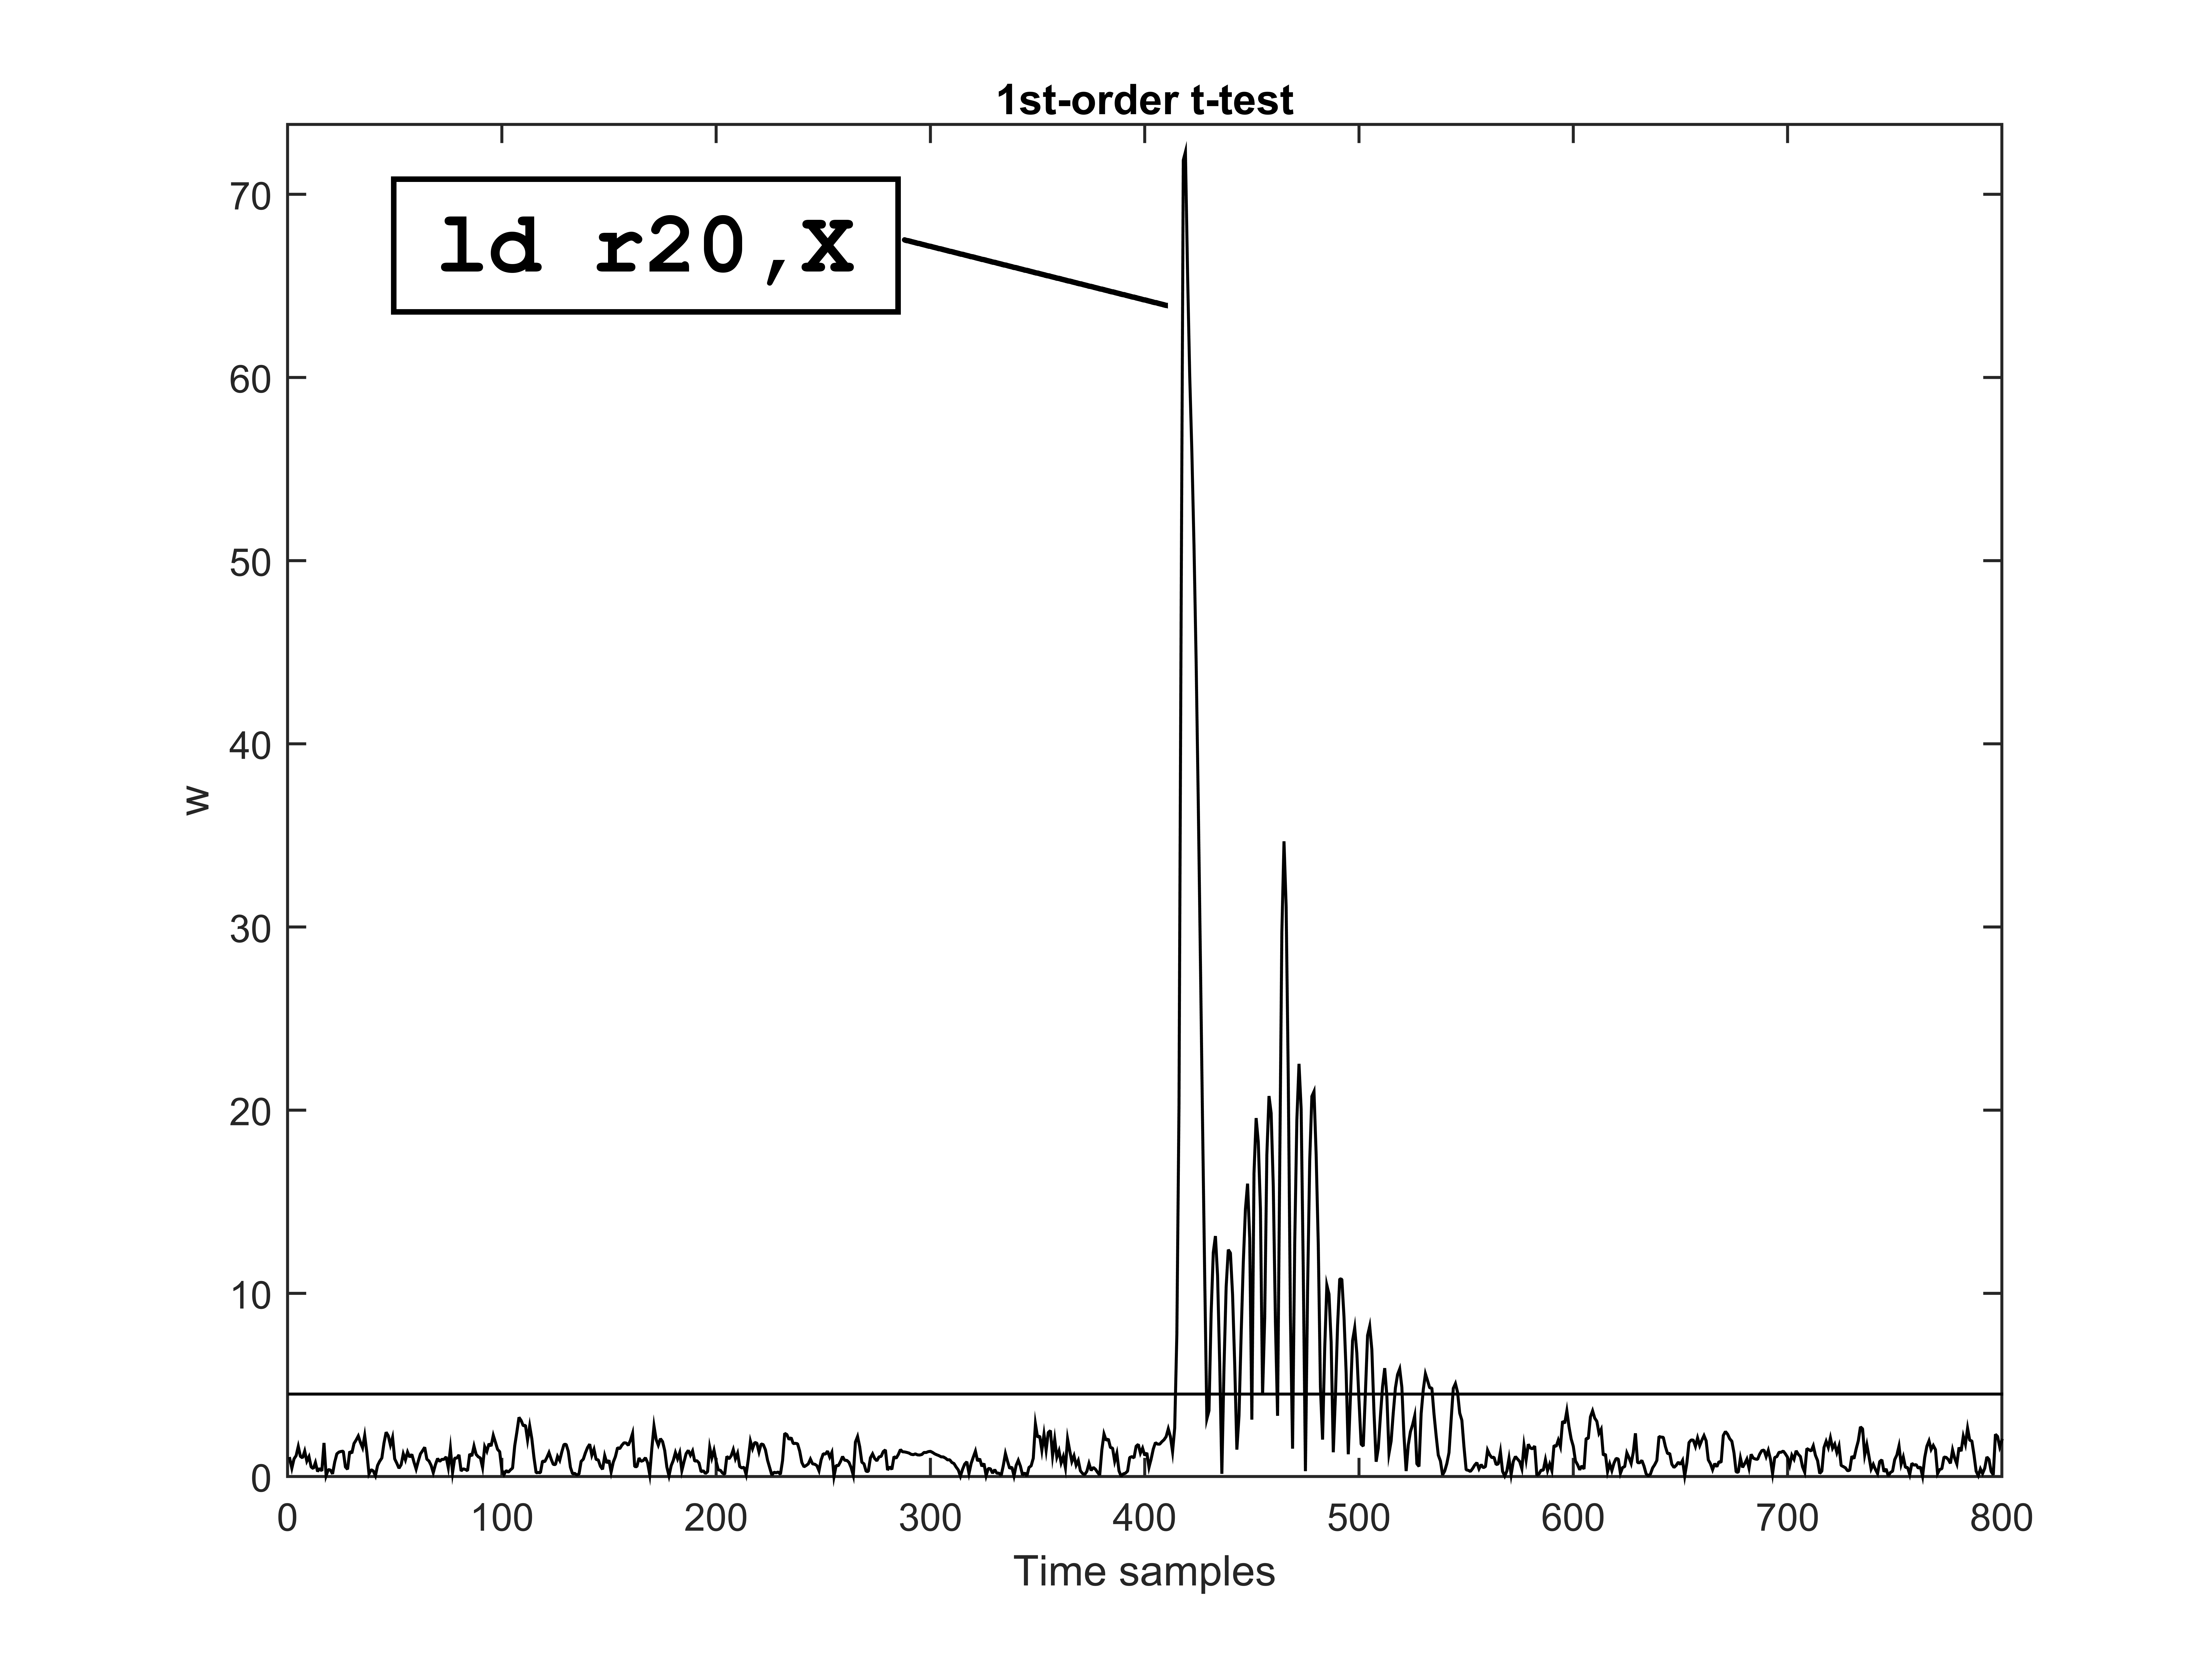
\includegraphics[width=\textwidth]{mem_rem_t_an.png}

        \caption{\scriptsize{Memory remnant effect, 1st-order t-test, 5k random vs. 5k fixed.}}

    \end{subfigure}
 \begin{subfigure}[b]{0.47\textwidth}
        %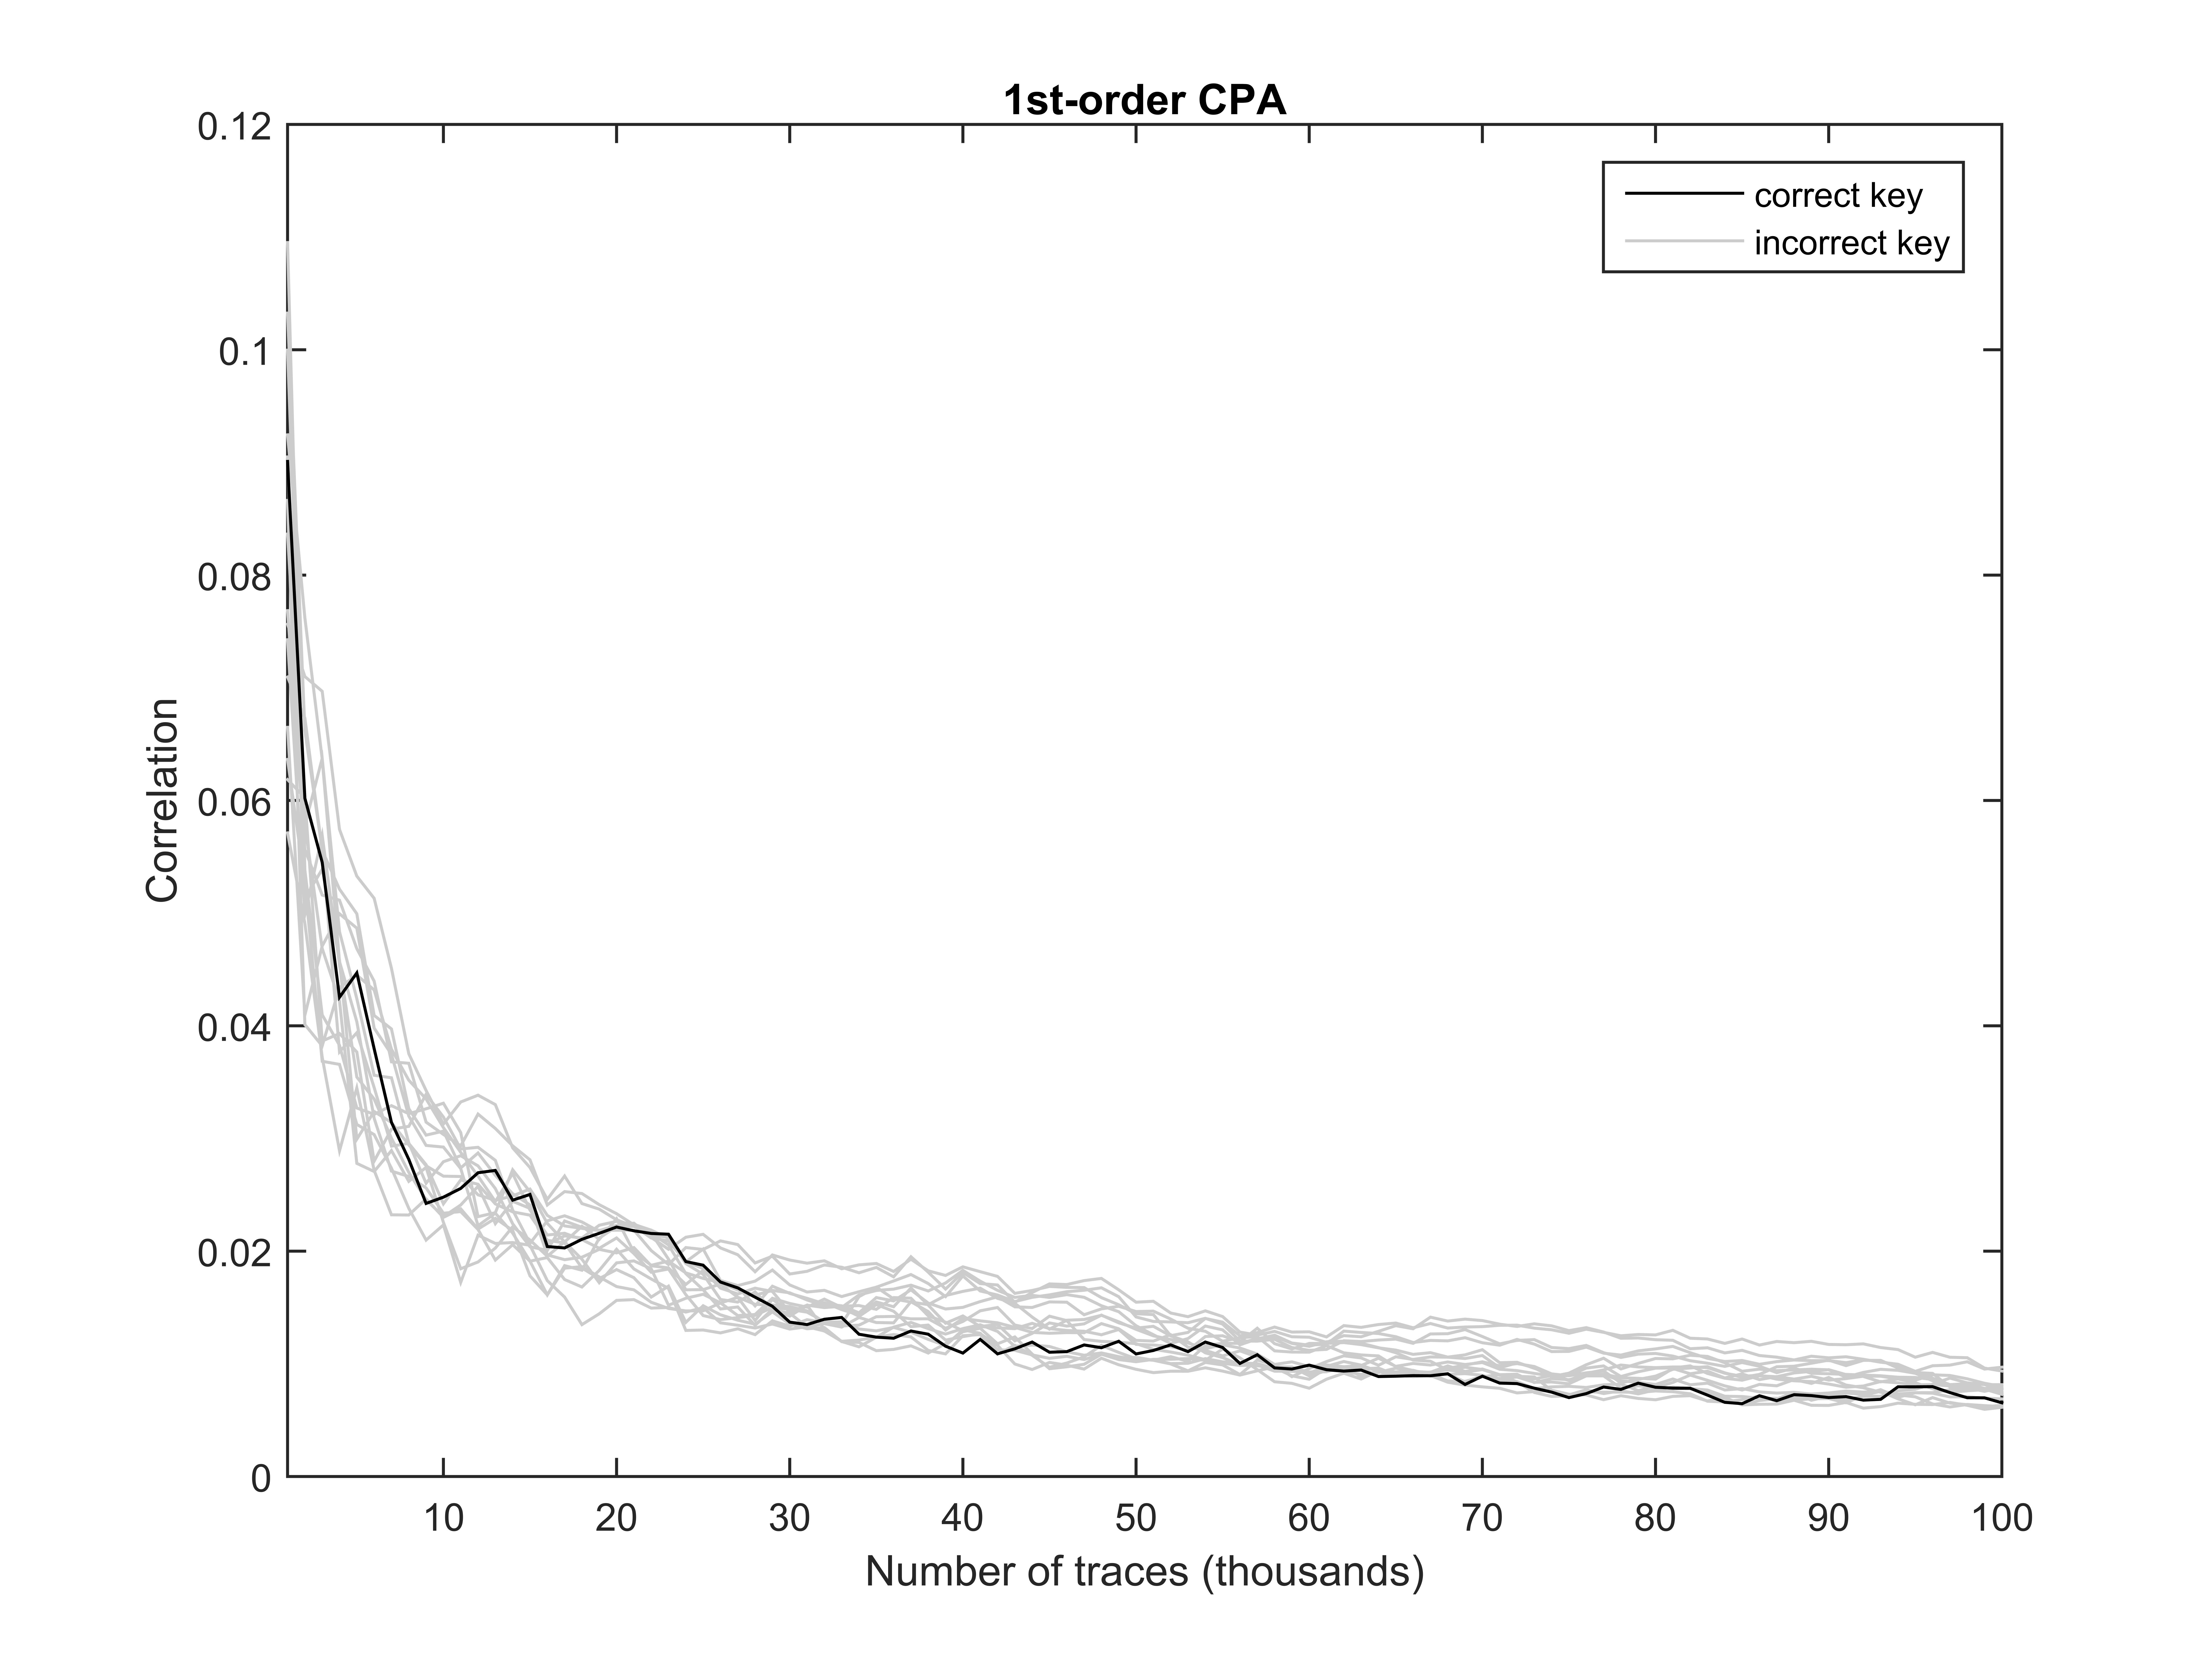
\includegraphics[width=\textwidth]{clear_rem_cpa.png}

        \caption{\scriptsize{Clearing remnant effect,1st-order CPA, HW model, 100k traces.}}

    \end{subfigure}
 \begin{subfigure}[b]{0.47\textwidth}
       %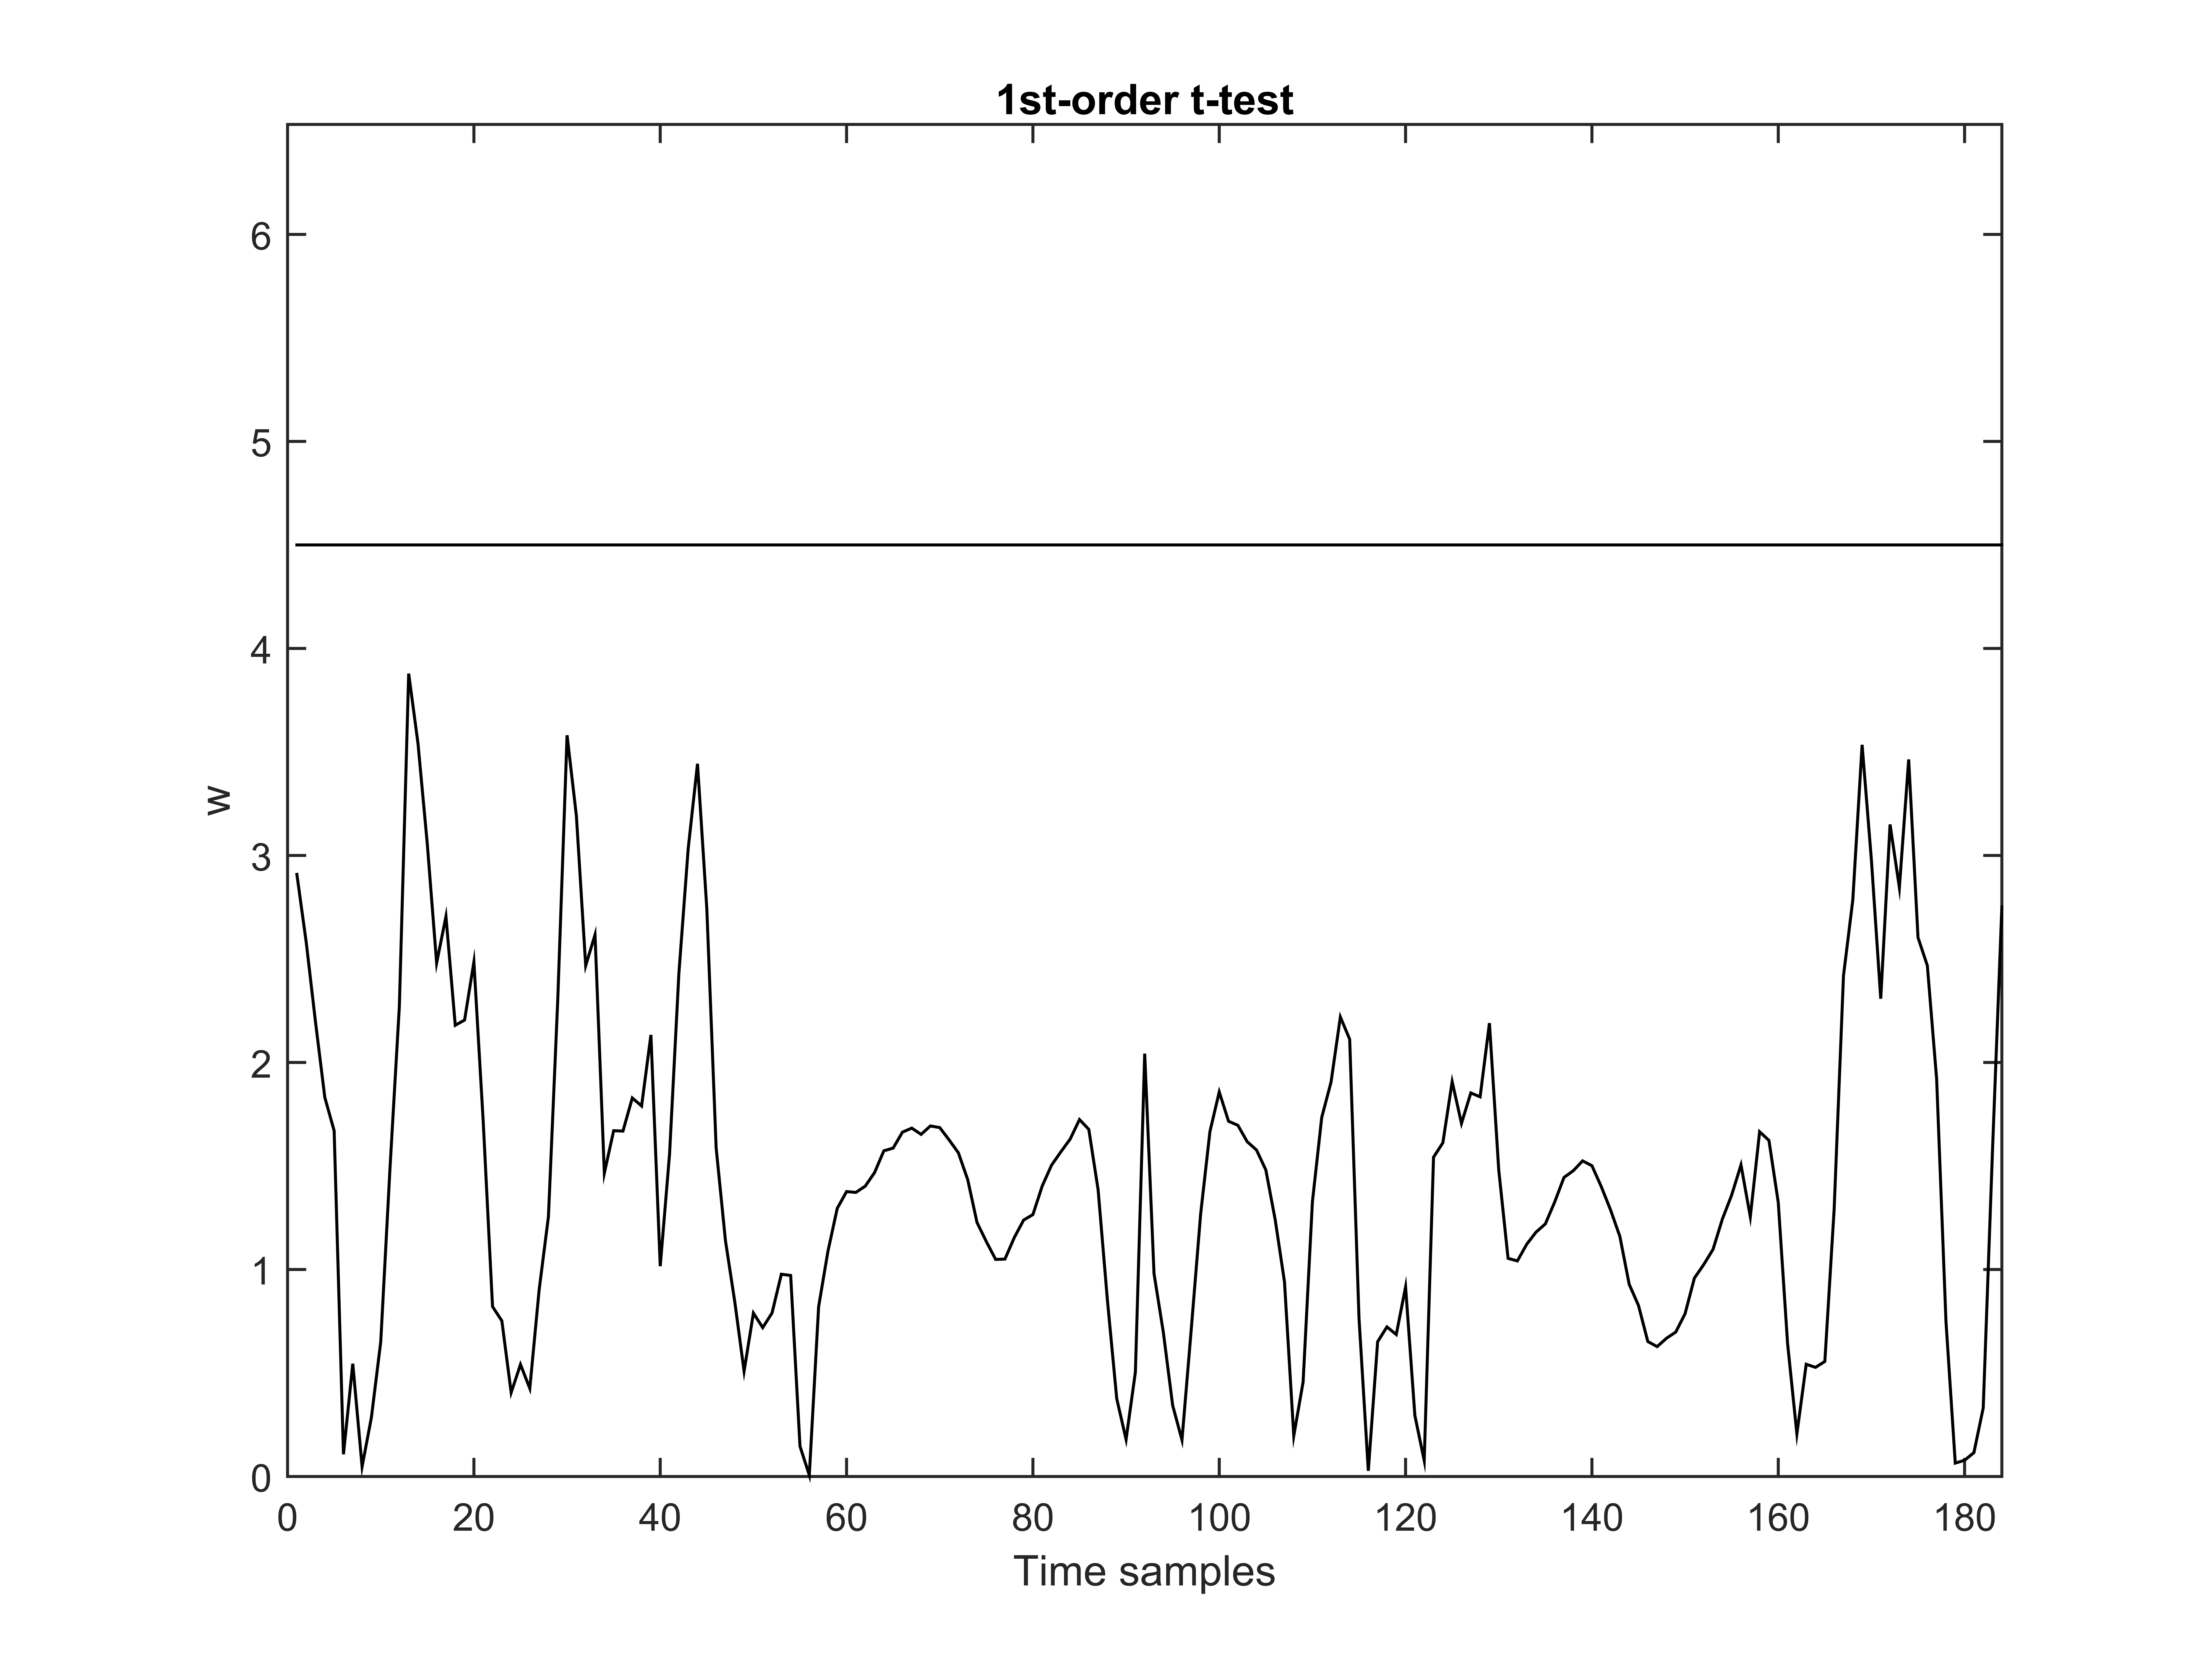
\includegraphics[width=\textwidth]{clear_rem_t.png}

        \caption{\scriptsize{Clearing remnant effect, 1st-order t-test, 100k random vs. 100k fixed.}}

    \end{subfigure}

   
    \caption{Memory remnant effect}\label{fig:regleak}
\end{figure}
As shown above, consecutive SRAM accesses can potentially lead to ILA violations. Preventing this requires the clearing of the register and the insertion of dummy SRAM. Alternatively, the implementor could ensure that same-family shares are not accessed sequentially. Exploiting (in a univariate manner) the memory remnant effect in ATMega163 requires less than 500 traces with our setup. The \texttt{st} instruction produces a similar effect (see Appendix A\todo{add appendix}).
\end{subsection}

\begin{subsection}{Combined Leakage Effect}\label{combined_leakage}

\todo[inline]{should we call this thing 'neighbour leakage effect'?}
The combined leakage effect implies that accessing or processing the contents of a data storage unit will cause leakage in another unit as well. For example, assume that share $x_0$ is stored in register \texttt{rB} and share $x_1$ is being processed in register \texttt{rA}. Assume also that the registers \texttt{rA, rB} are subject to the combined leakage effect. Processing \texttt{rB} will produce a value-based leakage of $x_1$. At the same time, the combined leakage effect will cause \texttt{rA} to leak the value of $x_0$, resulting in the concurrent leakage of both shares, revealing the sensitive value $x$.

The following two experiments verify the combined leakage effect between registers \texttt{r2, r3}, i.e. that a share stored in \texttt{r2} leaks when manipulating \texttt{r2} \emph{or} \texttt{r3} and vice-versa.
\begin{figure}[H]
    \centering
\begin{subfigure}[b]{0.4\textwidth}
\texttt{;clear all registers\\
;store x0 in r2 \\
mov r0, r0\\
NOPs \\
mov r1, r1\\
NOPs \\
mov r2, r2\\
NOPs \\
mov r3, r3 \\
NOPs \\
...\\
mov r31, r31 }

        \caption{\scriptsize{Combined leakage \texttt{r2-r3}.}}

    \end{subfigure}
\begin{subfigure}[b]{0.4\textwidth}
\texttt{;clear all registers\\
;store x0 in r3 \\
mov r0, r0\\
NOPs \\
mov r1, r1\\
NOPs \\
mov r2, r2\\
NOPs \\
mov r3, r3 \\
NOPs \\
...\\
mov r31, r31 }

        \caption{\scriptsize{Combined leakage \texttt{r3-r2}.}}

    \end{subfigure}


 \begin{subfigure}[b]{0.47\textwidth}
        %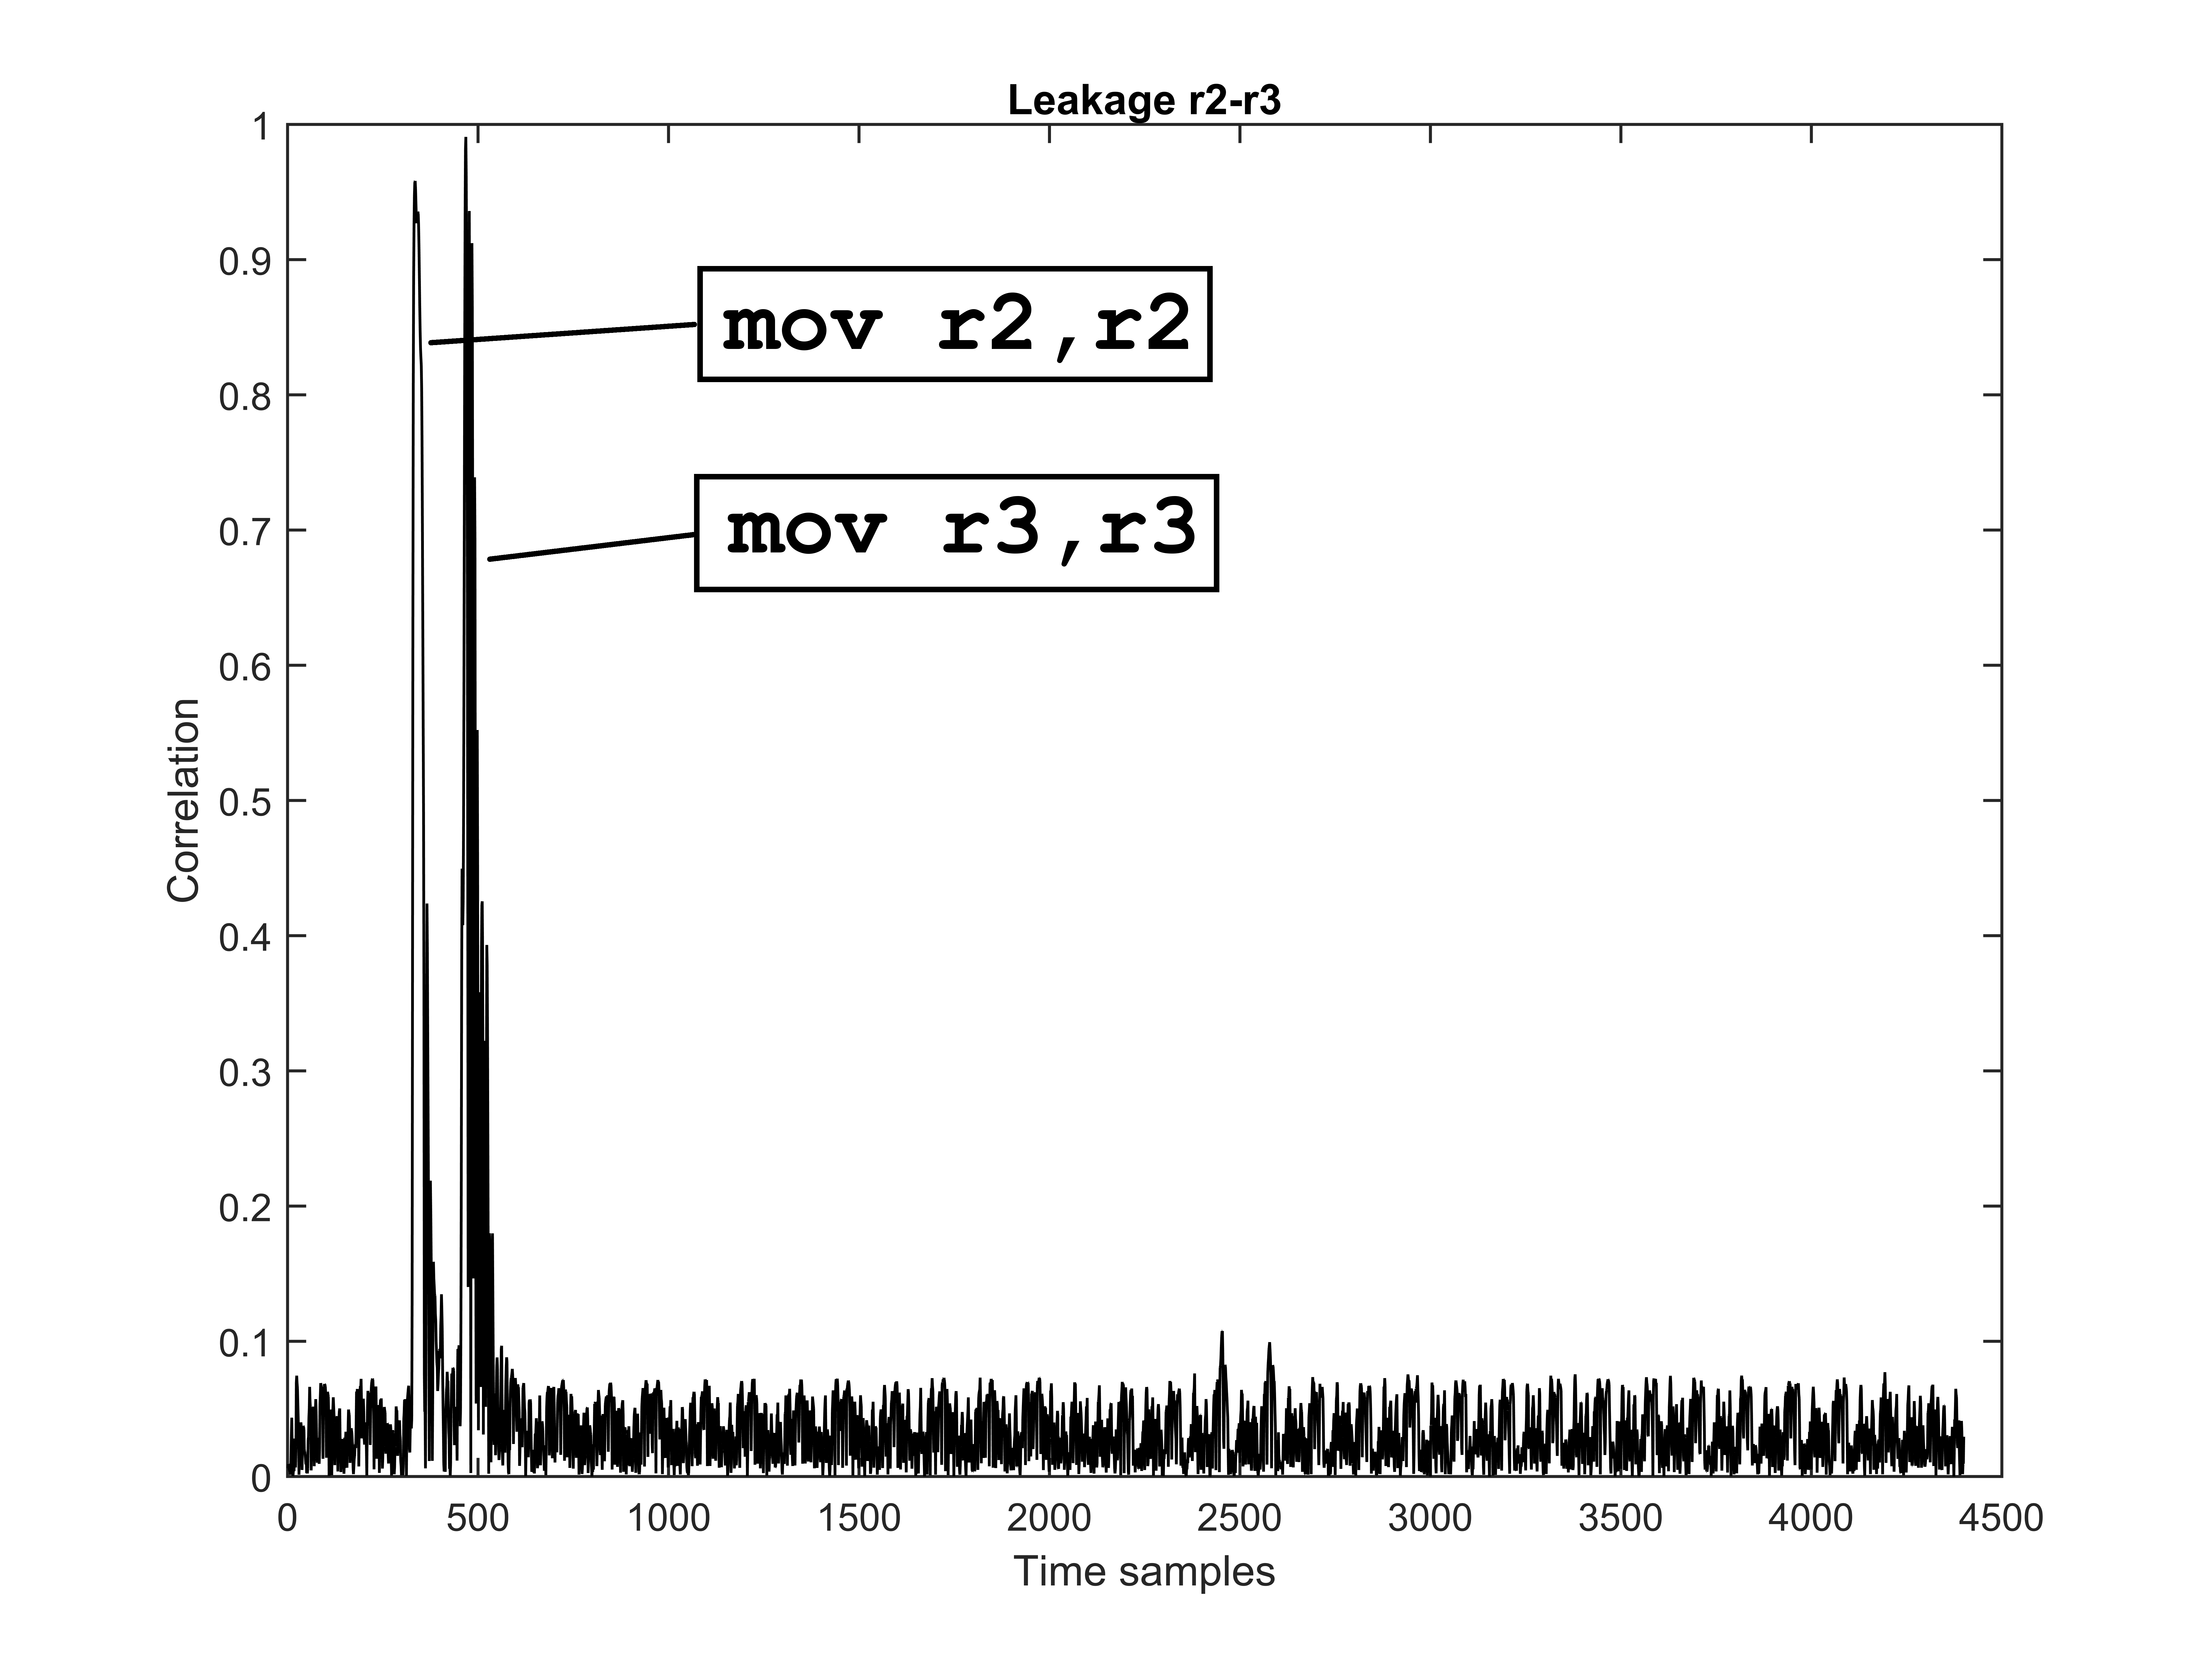
\includegraphics[width=\textwidth]{corr_r23_an.png}

        \caption{\scriptsize{Correlation \texttt{r2-r3} $\rho(HW(x_0),traceset)$, 5k traces.}}

    \end{subfigure}
 \begin{subfigure}[b]{0.47\textwidth}
        %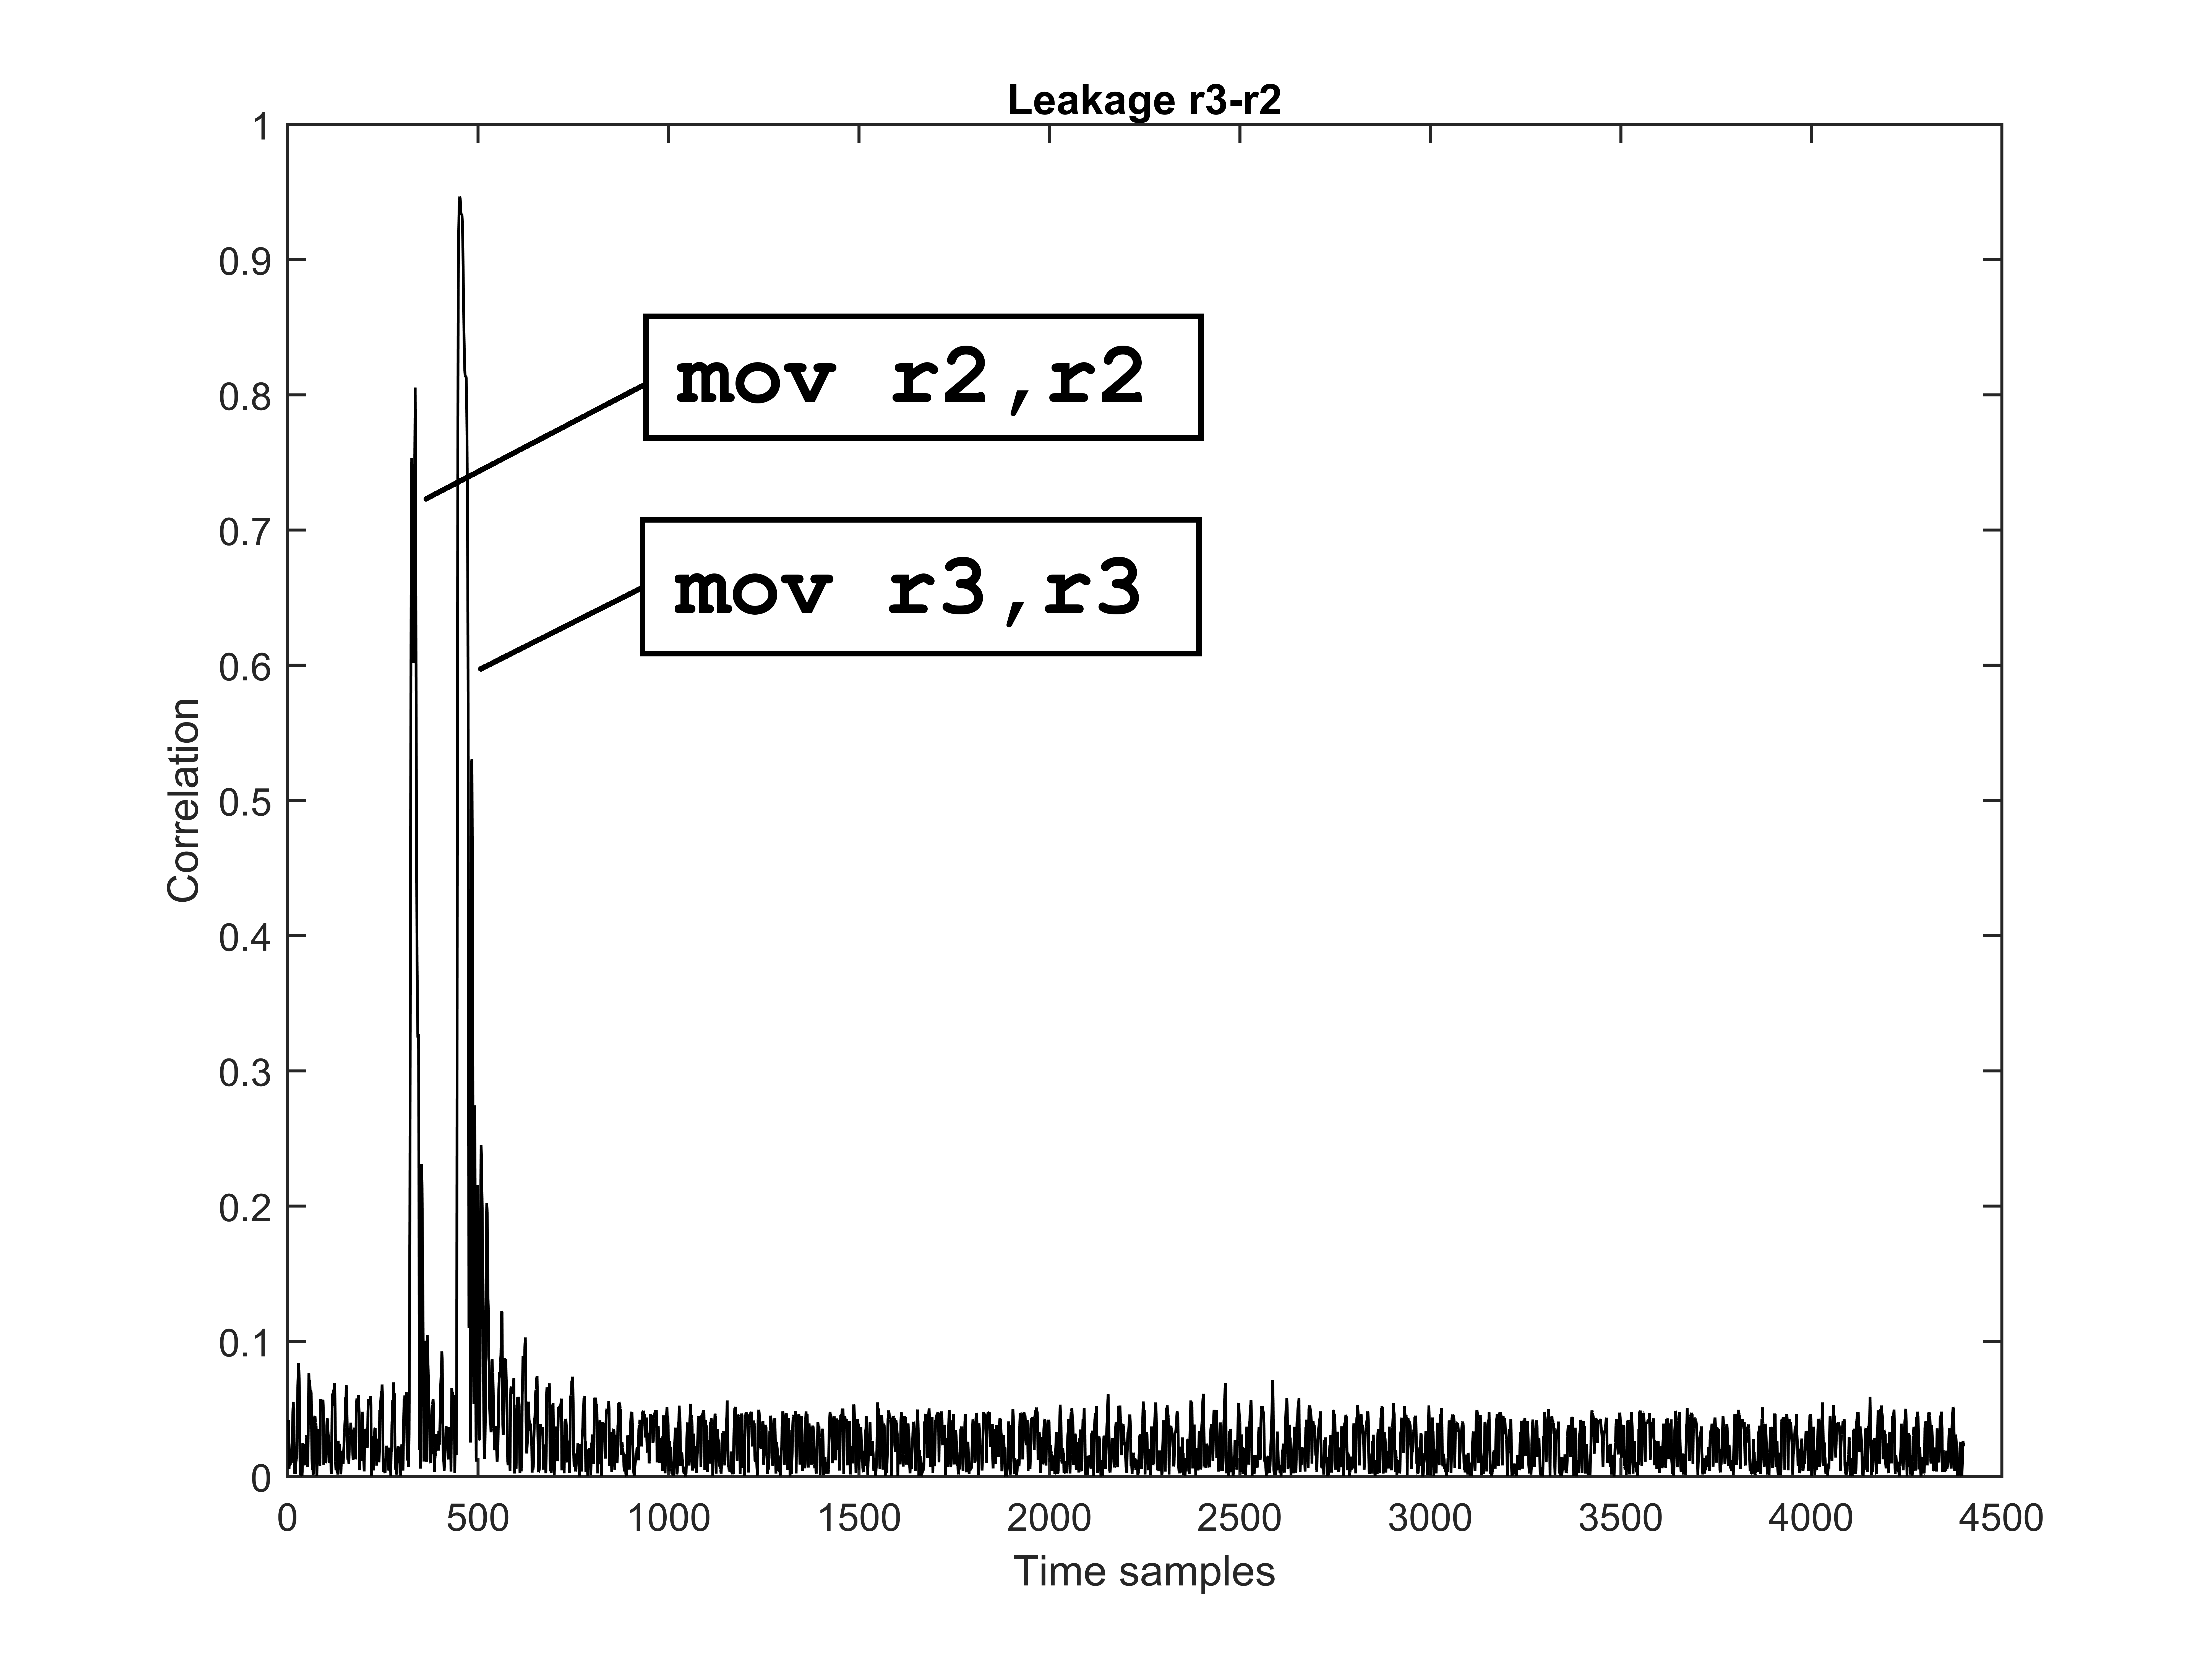
\includegraphics[width=\textwidth]{corr_r32_an.png}

        \caption{\scriptsize{Correlation \texttt{r3-r2} $\rho(HW(x_0),traceset)$, 5k traces.}}

    \end{subfigure}

   
    \caption{Combined leakage effect.}\label{fig:regleak}
\end{figure}


\end{subsection}
As shown above, we have identified a pair of data storage units (\texttt{r2,r3}) that exhibit the combined leakage effect. Note that in this case the effect is symmetrical, i.e. \texttt{r2} triggers \texttt{r3} and vice-versa. We run the same experiment in order to identify all possible combined leakages in the register file. The results are available in Appendix A\todo{add appendix}, matrix $R$. The combined leakage mostly affects neighboring registers, although exceptions exist, e.g. register \texttt{r0}. We did not identify a similar effect in SRAM memory cells, yet our experiments were limited to a small region of neighboring cells 

\begin{subsection}{Other Leakage Effects}
\todo[inline]{PENDING}

\end{subsection}


Summing up, we stress the following focal points regarding the ILA-breaching effects and their solutions:
\begin{itemize}
\item All identified effects are device-dependent, i.e. there is no hard guarantee that they are observable and reproducible in different AVR-based (or other instruction set) microcontrollers, let alone different architectures such as ARM, TI, PIC etc. Both intra-AVR and inter-architectural observability of the effects remains open.
\item The effects are often counter-intuitive when viewed in the assembly layer of abstraction. They originate from the hardware and/or the physical layer, thus can only be detected via experimental evaluation. Linking the assembly ILA-breaching effects to a particular hardware component or physical phenomenon is non-trivial~\cite{renauld,others}\todo{bib ref}, especially without knowledge of the underlying chip architecture and properties.
\item  Since the effect's detection requires experimental evaluation, different instructions or code arrangements can potentially lead to additional, unidentified ILA-breaching effects. Still, we maintain that it is possible to construct ``hardened" masked operations in ATMega163 by removing the identified effects (see Section \ref{sbox_section}). It remains open whether the suggested solutions are computationally optimal or more efficient clearing techniques can be identified.
\end{itemize}

The takeaway message of this section is that assembly-level soundness cannot enforce ILA and hence 1st-order security, due to the nature of the breaching effects. However, it is possible to acquire sufficient knowledge about effects and solutions in a particular device. These non-intuitive checks discussed above can be subsequently integrated into a code-checking tool which can identify such effects in assembly code.
